
\lstset{tabsize=2}
\chapter{PDDL}

\section{Blocks domain}\label{blocks}
\subsection{Problem Description}\label{blocks-prob}
\lstinputlisting{appendix/block-problem.pddl}
\subsection{Domain Description}\label{blocks-domain}
\lstinputlisting{appendix/blocks-domain.pddl}


\section{Domain Variation}\label{Domain_Variation}
The original part of the update domain and what its replaced with in the existential approach.
\subsection{Original}\label{domain}
\lstinputlisting{appendix/domain.txt}
\subsection{Changed}\label{domain2}
\lstinputlisting{appendix/domain2.txt}
\section{Levels}
{\huge insert levels here}

\chapter{Astro Kid}
\section{Astro Kid Rules}

The player can do the following things: walk left and right, climb up and down on ladders, and push objects horizontally away from it.
\section{Astro Kid Levels}
\begin{figure}
	\centering
	
	\caption{Level 25}
	\label{level25}
	
	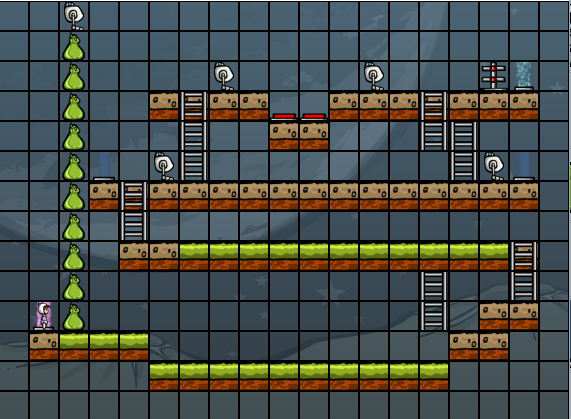
\includegraphics[width=1.0\textwidth]{appendix/img/lvl25}
\end{figure}
\begin{figure}
	\centering
	\caption{Level 31}
	\label{level31}
		
	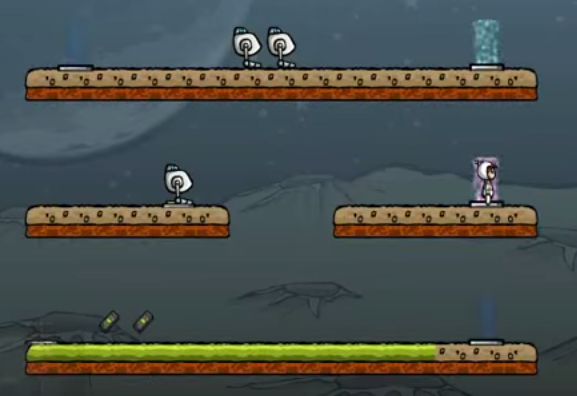
\includegraphics[width=1.0\textwidth]{appendix/img/lvl31}
\end{figure}
\begin{figure}
	\centering
	\caption{Toy problem 2}
	\label{prob02}
	
	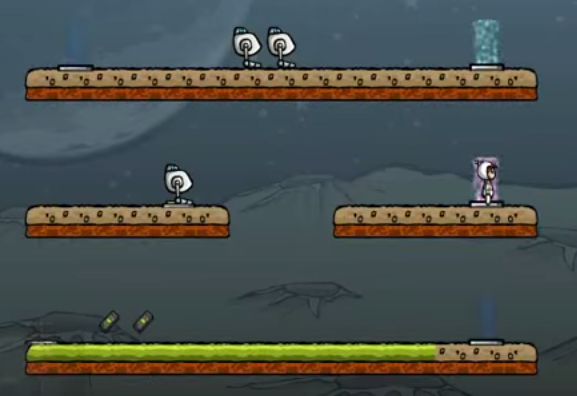
\includegraphics[width=1.0\textwidth]{appendix/img/lvl31}
\end{figure}